\documentclass[]{book}
\usepackage{lmodern}
\usepackage{amssymb,amsmath}
\usepackage{ifxetex,ifluatex}
\usepackage{fixltx2e} % provides \textsubscript
\ifnum 0\ifxetex 1\fi\ifluatex 1\fi=0 % if pdftex
  \usepackage[T1]{fontenc}
  \usepackage[utf8]{inputenc}
\else % if luatex or xelatex
  \ifxetex
    \usepackage{mathspec}
  \else
    \usepackage{fontspec}
  \fi
  \defaultfontfeatures{Ligatures=TeX,Scale=MatchLowercase}
\fi
% use upquote if available, for straight quotes in verbatim environments
\IfFileExists{upquote.sty}{\usepackage{upquote}}{}
% use microtype if available
\IfFileExists{microtype.sty}{%
\usepackage{microtype}
\UseMicrotypeSet[protrusion]{basicmath} % disable protrusion for tt fonts
}{}
\usepackage[margin=1in]{geometry}
\usepackage{hyperref}
\hypersetup{unicode=true,
            pdftitle={Note with R4DS},
            pdfborder={0 0 0},
            breaklinks=true}
\urlstyle{same}  % don't use monospace font for urls
\usepackage{natbib}
\bibliographystyle{plainnat}
\usepackage{color}
\usepackage{fancyvrb}
\newcommand{\VerbBar}{|}
\newcommand{\VERB}{\Verb[commandchars=\\\{\}]}
\DefineVerbatimEnvironment{Highlighting}{Verbatim}{commandchars=\\\{\}}
% Add ',fontsize=\small' for more characters per line
\usepackage{framed}
\definecolor{shadecolor}{RGB}{248,248,248}
\newenvironment{Shaded}{\begin{snugshade}}{\end{snugshade}}
\newcommand{\AlertTok}[1]{\textcolor[rgb]{0.94,0.16,0.16}{#1}}
\newcommand{\AnnotationTok}[1]{\textcolor[rgb]{0.56,0.35,0.01}{\textbf{\textit{#1}}}}
\newcommand{\AttributeTok}[1]{\textcolor[rgb]{0.77,0.63,0.00}{#1}}
\newcommand{\BaseNTok}[1]{\textcolor[rgb]{0.00,0.00,0.81}{#1}}
\newcommand{\BuiltInTok}[1]{#1}
\newcommand{\CharTok}[1]{\textcolor[rgb]{0.31,0.60,0.02}{#1}}
\newcommand{\CommentTok}[1]{\textcolor[rgb]{0.56,0.35,0.01}{\textit{#1}}}
\newcommand{\CommentVarTok}[1]{\textcolor[rgb]{0.56,0.35,0.01}{\textbf{\textit{#1}}}}
\newcommand{\ConstantTok}[1]{\textcolor[rgb]{0.00,0.00,0.00}{#1}}
\newcommand{\ControlFlowTok}[1]{\textcolor[rgb]{0.13,0.29,0.53}{\textbf{#1}}}
\newcommand{\DataTypeTok}[1]{\textcolor[rgb]{0.13,0.29,0.53}{#1}}
\newcommand{\DecValTok}[1]{\textcolor[rgb]{0.00,0.00,0.81}{#1}}
\newcommand{\DocumentationTok}[1]{\textcolor[rgb]{0.56,0.35,0.01}{\textbf{\textit{#1}}}}
\newcommand{\ErrorTok}[1]{\textcolor[rgb]{0.64,0.00,0.00}{\textbf{#1}}}
\newcommand{\ExtensionTok}[1]{#1}
\newcommand{\FloatTok}[1]{\textcolor[rgb]{0.00,0.00,0.81}{#1}}
\newcommand{\FunctionTok}[1]{\textcolor[rgb]{0.00,0.00,0.00}{#1}}
\newcommand{\ImportTok}[1]{#1}
\newcommand{\InformationTok}[1]{\textcolor[rgb]{0.56,0.35,0.01}{\textbf{\textit{#1}}}}
\newcommand{\KeywordTok}[1]{\textcolor[rgb]{0.13,0.29,0.53}{\textbf{#1}}}
\newcommand{\NormalTok}[1]{#1}
\newcommand{\OperatorTok}[1]{\textcolor[rgb]{0.81,0.36,0.00}{\textbf{#1}}}
\newcommand{\OtherTok}[1]{\textcolor[rgb]{0.56,0.35,0.01}{#1}}
\newcommand{\PreprocessorTok}[1]{\textcolor[rgb]{0.56,0.35,0.01}{\textit{#1}}}
\newcommand{\RegionMarkerTok}[1]{#1}
\newcommand{\SpecialCharTok}[1]{\textcolor[rgb]{0.00,0.00,0.00}{#1}}
\newcommand{\SpecialStringTok}[1]{\textcolor[rgb]{0.31,0.60,0.02}{#1}}
\newcommand{\StringTok}[1]{\textcolor[rgb]{0.31,0.60,0.02}{#1}}
\newcommand{\VariableTok}[1]{\textcolor[rgb]{0.00,0.00,0.00}{#1}}
\newcommand{\VerbatimStringTok}[1]{\textcolor[rgb]{0.31,0.60,0.02}{#1}}
\newcommand{\WarningTok}[1]{\textcolor[rgb]{0.56,0.35,0.01}{\textbf{\textit{#1}}}}
\usepackage{longtable,booktabs}
\usepackage{graphicx,grffile}
\makeatletter
\def\maxwidth{\ifdim\Gin@nat@width>\linewidth\linewidth\else\Gin@nat@width\fi}
\def\maxheight{\ifdim\Gin@nat@height>\textheight\textheight\else\Gin@nat@height\fi}
\makeatother
% Scale images if necessary, so that they will not overflow the page
% margins by default, and it is still possible to overwrite the defaults
% using explicit options in \includegraphics[width, height, ...]{}
\setkeys{Gin}{width=\maxwidth,height=\maxheight,keepaspectratio}
\IfFileExists{parskip.sty}{%
\usepackage{parskip}
}{% else
\setlength{\parindent}{0pt}
\setlength{\parskip}{6pt plus 2pt minus 1pt}
}
\setlength{\emergencystretch}{3em}  % prevent overfull lines
\providecommand{\tightlist}{%
  \setlength{\itemsep}{0pt}\setlength{\parskip}{0pt}}
\setcounter{secnumdepth}{5}
% Redefines (sub)paragraphs to behave more like sections
\ifx\paragraph\undefined\else
\let\oldparagraph\paragraph
\renewcommand{\paragraph}[1]{\oldparagraph{#1}\mbox{}}
\fi
\ifx\subparagraph\undefined\else
\let\oldsubparagraph\subparagraph
\renewcommand{\subparagraph}[1]{\oldsubparagraph{#1}\mbox{}}
\fi

%%% Use protect on footnotes to avoid problems with footnotes in titles
\let\rmarkdownfootnote\footnote%
\def\footnote{\protect\rmarkdownfootnote}

%%% Change title format to be more compact
\usepackage{titling}

% Create subtitle command for use in maketitle
\providecommand{\subtitle}[1]{
  \posttitle{
    \begin{center}\large#1\end{center}
    }
}

\setlength{\droptitle}{-2em}

  \title{Note with R4DS}
    \pretitle{\vspace{\droptitle}\centering\huge}
  \posttitle{\par}
    \author{}
    \preauthor{}\postauthor{}
      \predate{\centering\large\emph}
  \postdate{\par}
    \date{2019-05-17}

\usepackage{booktabs}

\begin{document}
\maketitle

{
\setcounter{tocdepth}{1}
\tableofcontents
}
\hypertarget{about-this-notebook}{%
\chapter*{About this notebook}\label{about-this-notebook}}
\addcontentsline{toc}{chapter}{About this notebook}

這本筆記本是我讀完\href{https://r4ds.had.co.nz}{\textbf{R for Data Science}}這本書後所嘗試使用\texttt{bookdown}所做的練習、以及這本書中練習題的解法。其中也參考了\href{https://bookdown.org/yihui/rmarkdown/}{\textbf{R Markdown: The Definitive Guide}}和\href{https://bookdown.org/yihui/bookdown/}{\textbf{bookdown: Authoring Books and Technical Documents with R Markdown}}這兩本書。

This notebook is my practice after reading those books:

\begin{itemize}
\tightlist
\item
  \href{https://r4ds.had.co.nz}{\textbf{R for Data Science}}
\item
  \href{https://bookdown.org/yihui/rmarkdown/}{\textbf{R Markdown: The Definitive Guide}}
\item
  \href{https://bookdown.org/yihui/bookdown/}{\textbf{bookdown: Authoring Books and Technical Documents with R Markdown}}
\end{itemize}

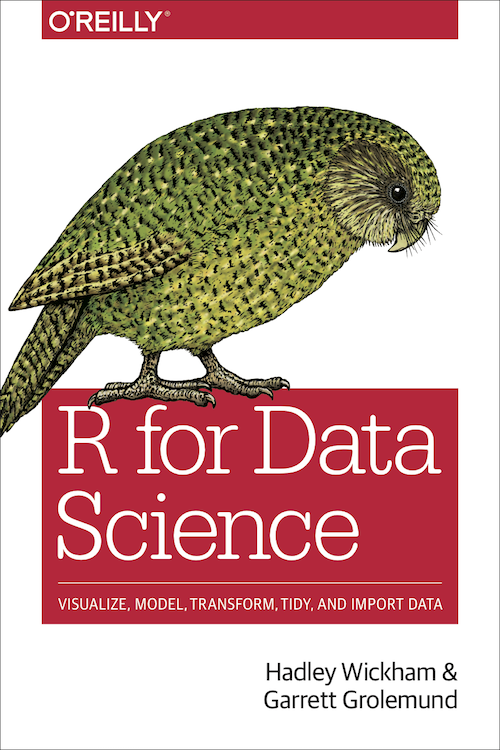
\includegraphics[width=0.33\linewidth]{images/f4ds}

\includegraphics[width=0.33\linewidth]{images/rmd}

\includegraphics[width=0.33\linewidth]{images/bookdown}

\hypertarget{intro}{%
\chapter{Introduction}\label{intro}}

Data science is an exciting discipline that allows you to turn raw data into understanding, insight, and knowledge. The goal of ``R for Data Science'' is to help you learn the most important tools in R that will allow you to do data science. After reading this book, you'll have the tools to tackle a wide variety of data science challenges, using the best parts of R.

\hypertarget{data-science-project-process}{%
\section{Data Science Project process:}\label{data-science-project-process}}

Data science is a huge field, and there's no way you can master it by reading a single book. The goal of this book is to give you a solid foundation in the most important tools. Our model of the tools needed in a typical data science project looks something like this:

\begin{center}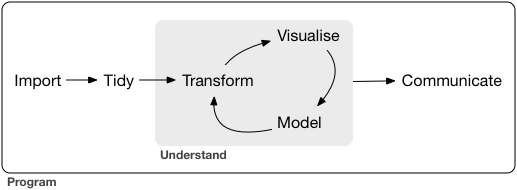
\includegraphics[width=1\linewidth]{images/data-science} \end{center}

\hypertarget{what-you-wont-learn}{%
\section{What you won't learn}\label{what-you-wont-learn}}

\begin{itemize}
\tightlist
\item
  Big Data
\item
  Python, Julia, and friends
\item
  Non-rectangular data
\item
  Hypothesis confirmation
\end{itemize}

\hypertarget{prerequisites}{%
\section{Prerequisites}\label{prerequisites}}

\hypertarget{r}{%
\subsection{R}\label{r}}

\begin{itemize}
\tightlist
\item
  Download R from CRAN: \url{https://cran.r-project.org}
\item
  Cloud mirror: \url{https://cloud.r-project.org} (which automatically figures it out for you.)
\end{itemize}

\hypertarget{rstudio}{%
\subsection{RStudio}\label{rstudio}}

\begin{itemize}
\tightlist
\item
  Download and install it from \url{http://www.rstudio.com/download}
\item
  RStudio IDE Cheat Sheet: \url{https://www.rstudio.com/resources/cheatsheets/\#ide}
\end{itemize}

\hypertarget{the-tidyverse-packages}{%
\subsection{The tidyverse packages}\label{the-tidyverse-packages}}

Install the tidyverse packages:

\begin{Shaded}
\begin{Highlighting}[]
\KeywordTok{install.packages}\NormalTok{(}\StringTok{"tidyverse"}\NormalTok{)}
\end{Highlighting}
\end{Shaded}

Load it with the library() function:

\begin{Shaded}
\begin{Highlighting}[]
\KeywordTok{library}\NormalTok{(tidyverse)}
\end{Highlighting}
\end{Shaded}

Update the packages:

\begin{Shaded}
\begin{Highlighting}[]
\KeywordTok{tidyverse_update}\NormalTok{()}
\end{Highlighting}
\end{Shaded}

\hypertarget{other-packages}{%
\subsection{Other packages}\label{other-packages}}

In this book we'll use three data packages from outside the tidyverse:

\begin{Shaded}
\begin{Highlighting}[]
\KeywordTok{install.packages}\NormalTok{(}\KeywordTok{c}\NormalTok{(}\StringTok{"nycflights13"}\NormalTok{, }\StringTok{"gapminder"}\NormalTok{, }\StringTok{"Lahman"}\NormalTok{))}
\end{Highlighting}
\end{Shaded}

\hypertarget{introduction}{%
\chapter{Introduction}\label{introduction}}

\hypertarget{data-visualisation}{%
\chapter{Data visualisation}\label{data-visualisation}}


\end{document}
